\documentclass{article}
\usepackage[left=2cm,right=2cm,top=2cm,bottom=2cm]{geometry}
\usepackage{amsmath}
\usepackage{tikz}
\usepackage{hyperref}
\usepackage{venndiagram}
\usepackage{amssymb}
\usepackage{enumitem}
\usepackage{setspace}
\usepackage{amsthm}

\newtheorem{theorem}{Theorem}[section]
\newtheorem{lemma}{Lemma}[theorem]
\newtheorem{corollary}{Corollary}[theorem]

\theoremstyle{definition} 
\newtheorem{defi}{Definition}[section]
\newtheorem{exa}{Example}[defi]
\newtheorem{exe}{Exercise}
\newtheorem{sol}{Solution}[exe]
\newtheorem{pro}{Properties}[section]


\linespread{1.5}


\title{Eigenvalue and Eigenvector}
\author{Len Fu}
\date{11.27.2024}

\begin{document}

\maketitle

\tableofcontents

\newpage

\section{Exercise}
% \begin{exe}[0.3.6]
%     Prove:
%     \begin{enumerate}
%         \item A\cap (B\cup C)=(A\cap B)\cup (A\cap C).
%         \item A\cup (B\cap C)=(A\cup B)\cap (A\cup C).
%     \end{enumerate}
% \end{exe}
\begin{sol}[0.3.6]
For the first one, we suppose for all $x\in (A\cap B)\cup (A\cap C)$, then $x$ is in $A$ and in $B$ or $C$.
Now we consider two cases:
\begin{enumerate}
    \item If $x$ is in $A$ and $B$, then $x\in A\cap B$ and $x\in A\cap C$, then $x\in (A\cap B)\cup (A\cap C)$.
    \item If $x$ is in $A$ and $C$, then $x\in A\cap B$ and $x\in A\cap C$, then $x\in (A\cap B)\cup (A\cap C)$.
\end{enumerate}
Thus we have $(A\cap B)\cup (A\cap C)\subseteq A\cap (B\cup C)$.
Then we consider all $x\in A\cap (B\cup C)$, that $x$ is in $A$ or in $B$ and $C$.
\begin{enumerate}
    \item If $x$ is in $A$, then $x\in A\cap B$ and $x\in A\cap C$, then $x\in (A\cap B)\cup (A\cap C)$.
    \item If $x$ is in $B$ and $C$, then $x\in A\cap B$ and $x\in A\cap C$, then $x\in (A\cap B)\cup (A\cap C)$.
\end{enumerate}
Thus we have $A\cap (B\cup C)\subseteq (A\cap B)\cup (A\cap C)$ and we have $ A\cap (B\cup C)=(A\cap B)\cup (A\cap C)$.

For the second one, we suppose for all $x\in (A\cup B)\cap (A\cup C)$, then $x$ is in $A$ and $B$ or in $A$ and $C$.
\begin{enumerate}
    \item If $x$ is in $A$ and $B$, then $x\in A$, then $x\in A\cup (B\cap C)$.
    \item If $x$ is in $A$ and $C$, then $x\in A$, then $x\in A\cup (B\cap C)$.
\end{enumerate}
Thus we have $(A\cup B)\cap (A\cup C)\subseteq A\cup (B\cap C)$.
Then we consider all $x\in A\cup (B\cap C)$, that $x$ is in $A$ or in $B$ and $C$.
\begin{enumerate}
    \item If $x$ is in $A$, then $x\in A\cup B$ and $x\in A\cup C$, then $x\in (A\cup B)\cap (A\cup C)$.
    \item If $x$ is in $B$ and $C$, then $x\in B$ and $x\in C$, then $x\in A\cup B$ and $x\in A\cup C$, then $x\in (A\cup B)\cap (A\cup C)$.
\end{enumerate}
Thus we have $A\cup (B\cap C)\subseteq (A\cup B)\cap (A\cup C)$ and we have $ A\cup (B\cap C)=(A\cup B)\cap (A\cup C)$.
\end{sol}

\begin{sol}[0.3.7]
\begin{enumerate}
    \item There is the venndiagram of the $A\Delta B$:\\
    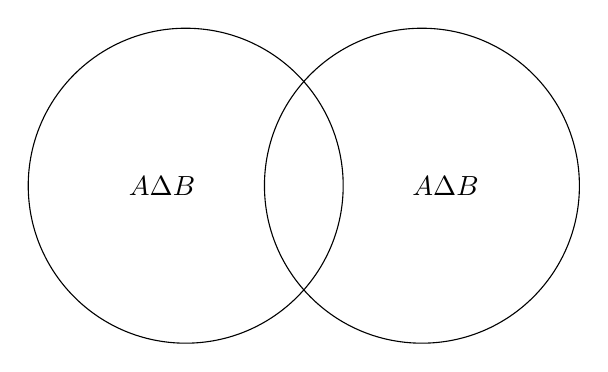
\begin{tikzpicture}
        \draw (0,0) circle (2cm) ;
        \draw (3,0) circle (2cm) ;
        \node at (3.3,0) {$A \Delta B$};
        \node at (-0.3,0) {$A\Delta B$};
      \end{tikzpicture}
    \item For all $x\in A\Delta B$, then $x$ is in $A$ or $B$ but not in $A$ and $B$.
    \begin{enumerate}[label=(\alph*)]
        \item If $x$ is in $A$ but not in $B$ and $A$, then $x\in A\setminus B$ and $x\in(A\setminus B)\cup (B\setminus A)$.
        \item If $x$ is in $B$ but not in $B$ and $A$, then $x\in B\setminus A$ and $x\in(A\setminus B)\cup (B\setminus A)$.
    \end{enumerate}
    Thus we have $A\Delta B\subseteq (A\setminus B)\cup (B\setminus A)$.
    Inversely, for all $x\in (A\setminus B)\cup (B\setminus A)$, then :
    \begin{enumerate}[label=(\alph*)]
        \item If $x$ is in $A\setminus B$, then $x\in A$ and $x\notin B$, then $x\in A\Delta B$.
        \item If $x$ is in $B\setminus A$, then $x\in B$ and $x\notin A$, then $x\in A\Delta B$.
    \end{enumerate}
    Thus we have $(A\setminus B)\cup (B\setminus A)\subseteq A\Delta B$.
    Thus we have $A\Delta B=(A\setminus B)\cup (B\setminus A)$.
    \item For all $x\in A\Delta B$, then $x$ is in $A$ or $B$ but not in $A$ and $B$.
    \begin{enumerate}[label=(\alph*)]
        \item If $x$ is in $A$ but not in $B$ and $A$, then $x\in A\cup B$ and $x\notin (A\cap B)$, then $x\in (A\cup B)\setminus (A\cap B)$.
        \item If $x$ is in $B$ but not in $B$ and $A$, then $x\in A\cup B$ and $x\notin (A\cap B)$, then $x\in (A\cup B)\setminus (A\cap B)$.
    \end{enumerate}
    Thus we have $A\Delta B\subseteq (A\cup B)\setminus (A\cap B)$.
    Inversely, for all $x\in (A\cup B)\setminus (A\cap B)$, then $x$ is in $A$ but not in $B$ and $A$, or 
    $x$ is in $B$ but not in $B$ and $A$, then $x\in A\Delta B$.
    Thus we have $(A\cup B)\setminus (A\cap B)\subseteq A\Delta B$.
    Thus we have $A\Delta B=(A\cup B)\setminus (A\cap B)$.

\end{enumerate}
\end{sol}

\begin{sol}[0.3.8]
    \begin{enumerate}[label=(\alph*)]
        \item $\left\{6k|k\in\mathbb{N}\right\}$.
        \item $\left\{k|k\in\mathbb{N}\ but\ k\neq 1\right\}$
        \item $\left\{0\right\}$
    \end{enumerate}
\end{sol}

\begin{sol}[0.3.14]
Using principle of induction, we have:

    \noindent\textbf{Basis statement:}For n=1, left side is 1, right side is 1, thus the statement is true.

    \noindent\textbf{Induction step:}Suppose the statement is true for $n=k$, then we have:
    $$1^{3}+2^{3}+\cdots+k^{3}=(\frac{k(k+1)}{2})^{2}.$$
    Now consider $n=k+1$, since 
    \begin{align*}
        (\frac{(k+1)(k+1+1)}{2})^{2}-(\frac{k(k+1)}{2})^{2}=\frac{k^{4}+6k^{3}+13k^{2}+2k+4-(k^{4}+2k^{3}+k^{2})}{4}=k^{3}+3k^{2}+3K+1\\
        1^{3}+2^{3}+\cdots+k^{3}+(k+1)^{3}=(\frac{k(k+1)}{2})^{2}+(\frac{(k+1)(k+1+1)}{2})^{2}-(\frac{k(k+1)}{2})^{2}\\
        1^{3}+2^{3}+\cdots+k^{3}+(k+1)^{3}=(\frac{(k+1)(k+2)}{2})^{2}
    \end{align*}
    Thus we have the statement is true for $n=k+1$, thus the statement is true for all $n\in\mathbb{N}$.
\end{sol}


\begin{sol}[0.3.15]
Using principle of induction, we have:

    \noindent\textbf{Basis statement:} For n=1, $n^{3}+5n\equiv 0(mod\ 6)$.

    \noindent\textbf{Induction step:} Suppose the statement is true for $n=k$, then we have:
    $$k^{3}+5k\equiv 0(mod\ 6).$$
    Now consider $n=k+1$, since
    \begin{align*}
        &(k+1)^{3}+5(k+1)\\
        =&k^{3}+5k+6+3k(k+1)\\
        &k^{3}+5k+6+3k(k+1)(mod\ 6)\\
        \equiv &(k^{3}+5k)(mod\ 6)+0+3k(k+1)(mod\ 6)\\
        \equiv &0+3k(k+1)(mod\ 6)\\
        \equiv &k(k+1)(mod\ 2)
    \end{align*}
    Actually $k(k+1)\equiv 0(mod\ 2)$ for all $k\in \mathbb{N}$, then we have 
    $$(k+1)^{3}+5(k+1)\equiv 0(mod\ 6).$$
    Thus we have the statement is true for $n=k+1$, thus the statement is true for all $n\in\mathbb{N}$.
\end{sol}

\begin{sol}[0.3.16]

    Define $f(n)=n^{3}-2(n+5)^{2},\ n\in\mathbb{N}$, and suppose $n_{0}$ is the smallest integer such that $f(n)>0$.Using principle of induction, we have:
    \\\noindent\textbf{Basis statement:} For $n=n_{0}$, $f(n)>0$, the statement is ture.
    \\\noindent\textbf{Induction step:} Suppose the statement is true for $n=k$, then we have:
    $$f(k)=k^{3}-2k^{2}-20k-50>0.$$
    Now consider $n=k+1$, since
    \begin{align*}
        f(k+1)=&(k+1)^{3}-2(k+1)^{2}-20(k+1)-50\\
        =&k^{3}+3k^{2}+3k+1-2k^{2}-4k-2-20k-20-50\\
        =&k^{3}-2k^{2}-20k-50+3k^{2}-k-21\\
    \end{align*}
    Obviously, $3<n_{0}$ and $3<k$, and $3k^{2}-k-21>3*3^{2}-3-21=3>0$, thus
    $$f(k+1)>0+0=0.$$
    Thus we have the statement is true for $n=k+1$, thus the statement is true for all $n\geq n_{0}$. 
\end{sol}

\begin{sol}[0.3.17]
    $$\left\{n|n\geq 2\ and\ n\in\mathbb{N}\right\}$$
\end{sol}

\begin{sol}[0.3.18]
    Using principle of strong induction, we consider a subset $S_{n}$ of $\mathbb{N}$ with $n$ elements, now:"
    
    \noindent\textbf{Basis statement:} For $n=1$, the element is the smallest element, then the statement is true for n=1.

    \noindent\textbf{Strong induction step:} Suppose the statement is true for $n=k$, then there exists a smallest element $x_{k}$ in $S_{k}$, and now we insert an element $a_{k+1}$ into the set $S_{k}$ as $S_{k+1}$.
    And $x_{k}$ or $a_{k+1}$ is the smallest element, then there exists a smallest element in $S_{k+1}$,then the statement is true for $n=k+1$.

\end{sol}
































\end{document}